\documentclass[10pt]{beamer}

\usetheme[sectionpage=none, progressbar=frametitle]{metropolis}

\definecolor{alertblue}{RGB}{0,110,191}
\definecolor{DarkGray}{RGB}{51,51,51}
\definecolor{RedAlert}{RGB}{255,0,0}

\setbeamercolor{progress bar}{fg=alertblue,bg=fg!50!black!30}
\setbeamercolor{normal text}{fg=DarkGray}
\setbeamercolor{alerted text}{fg=RedAlert}

%% =============================================================================
%%
%%                                      PACOTES
%%
%% =============================================================================

\usepackage[utf8]{inputenc}
\usepackage[brazil]{babel}
\usepackage{booktabs}
\usepackage[scale=2]{ccicons}
\usepackage{pgfplots}
\usepgfplotslibrary{dateplot}
\usepackage{xspace}
\usepackage{amsmath}
\usepackage{tikz}
\usepackage{multirow}
\usepackage{upgreek}
\usetikzlibrary{calc}
\usepackage[type={CC},modifier={by-nc-sa},version={4.0},]{doclicense}
\newcommand{\themename}{\textbf{\textsc{metropolis}}\xspace}


%% =============================================================================
%%
%%                                      INFOS
%%
%% =============================================================================


\title{Fundamentos de Escoamentos Reativos Turbulentos}
\subtitle{Aula 4 - 5}
\date{19 de setembro de 2016}
\author{Prof. Dr. Guenther Carlos Krieger Filho}
\institute{Escola Politécnica da USP - LETE/CRC - Combustion Research Centre}
\titlegraphic{
\includegraphics[height=1.0cm]{Logo-LETE_1.png}\hfill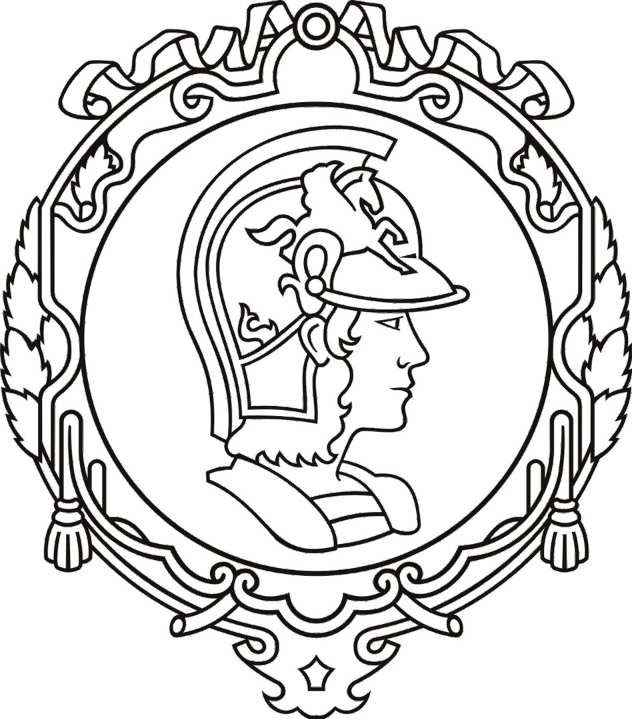
\includegraphics[height=1.5cm]{logo.png}}

%================================ USER DEFINED ==================================

\newcommand{\ddt}[1]{\dfrac{\partial #1}{\partial t}}
\newcommand{\tgrad}[1]{\dfrac{\partial #1}{\partial x_j}}

\newcommand{\ddx}[2]{\dfrac{\partial #1}{\partial x_{#2}}}
\newcommand{\ddxsp}[1]{\dfrac{\partial}{\partial x_{#1}}}

\newcommand{\ddxp}[2]{\dfrac{\partial }{\partial x_{#2}}\left(#1\right)}
\newcommand{\laplace}[1]{\dfrac{\partial^2 #1}{\partial x_{j}\partial x_{j}}}
\newcommand{\m}[1]{\overline{#1}}
\newcommand{\divr}[1]{\nabla \cdot #1}
\newcommand{\divp}[1]{\nabla \cdot \left(#1\right)}
\newcommand{\blue}[1]{{\color{blue}#1}}
\newcommand\incircle[1]{\tikz[baseline=(X.base)] \node(X)[draw, shape=circle, inner sep=0]{\strut #1};}
%=========================================              =========================================
\metroset{block=fill}
\begin{document}

%% =============================================================================
%%
%%                                      TITULO
%%
%% =============================================================================
\maketitle

%\begin{frame}{Conteudo}
%  \setbeamertemplate{section in toc}[sections numbered]
%  \tableofcontents[hideallsubsections]
%\end{frame}

\section{Introduction}

\begin{frame}{Momentum Conservation Equation}
	For an reactive multicomponent mixture, the momentum equation reads
	
	\begin{equation}
	\frac{\partial \rho u_{i}}{\partial t}+\frac{\partial \rho u_{i} u_{j}}{\partial x_{j}}=-\frac{\partial p}{\partial x_{i}}+\frac{\partial}{\partial x_{j}}\left[ 2 \mu S_{ij}-\frac{2}{3} \delta_{ij} \left( \mu \frac{\partial u_{k}}{\partial x_{k}}\right) \right] +\rho g_{i} +\rho\sum_{k=1}^N Y_{k}f_{k,i},
	\label{eq:ns1}
	\end{equation}
	
	\noindent where
	
	\begin{equation}\label{eq:deform}
	S_{ij}=\frac{1}{2}\left(\frac{\partial u_{i}}{\partial x_{j}}+\frac{\partial u_{j}}{\partial x_{i}}\right) ,
	\end{equation}
	
	The last term stands for the body force $f_{k}$ acting over the specie $k$ in the direction $i$. This could be, for example, electric/magnetic fields.
\end{frame}



\frame{\frametitle{Momentum Conservation Equation} 

	Neglecting the body forces, the averaged momentum equations reads

	\begin{equation}\label{eq:ns2}
	\frac{\partial \rho \overline{u}_{i} \overline{u}_{j}}{\partial x_{j}}=-\frac{\partial \overline{p}}{\partial x_{i}}+\frac{\partial}{\partial x_{j}}\left[  \mu \left(\frac{\partial \overline{u_{i}}}{\partial x_{j}}+\frac{\partial \overline{u}_{j}}{\partial x_{i}}\right)-\frac{2}{3} \delta_{ij} \left( \mu \frac{\partial \overline{u}_{k}}{\partial x_{k}}\right) \right] - \frac{\partial\rho\overline{u_{i}^{'}}\overline{u_{j}^{'}}}{\partial x_{i}} ,
	\end{equation}
	
	The last term stands for the Reynolds Stresses.
}


\frame{\frametitle{Classical Turbulence Models for the Reynolds Stresses} 

	\noindent With the analogy to the molecular viscous tensor, the Boussinesq assumption leads to
	
	\begin{equation}\label{eq:ns3}
	\rho\overline{u_{i}^{'}}\overline{u_{j}^{'}} =-\mu_{t}\left[   \left(\frac{\partial \overline{u_{i}}}{\partial x_{j}}+\frac{\partial \overline{u_{j}}}{\partial x_{i}}\right)-\frac{2}{3} \delta_{ij} \left( \frac{\partial \overline{u_{k}}}{\partial x_{k}}\right) \right] + \frac{2}{3}\delta_{ij}\rho k   ,
	\end{equation}
	
	where $k$ is the kinetic energy of the turbulence, defined as $k = \frac{1}{2}\overline{u_{i}^{'}u_{i}^{'}}$ 
	
	\noindent The question is, however, how to evaluate the turbulent viscosity $\mu_{t}$
}

\frame{\frametitle{Classical Turbulence Models : Zero Equation or Prandtl Mixing Length} 
	Prandtl has proposed to evaluate the turbulent viscosity based on the velocity gradient and a characteristic length $l_m$ as
	
	\begin{equation}
	\mu_{t}=\rho {l_m}^2 |\overline{S_{ij}}|
	\label{eq:mtPr}
	\end{equation}
	
	
	where
	
	\begin{equation}\label{eq:deformmean}
	\overline{S_{ij}}=\frac{1}{2}\left(\frac{\partial \overline{u_{i}}}{\partial x_{j}}+\frac{\partial \overline{u_{j}}}{\partial x_{i}}\right) ,
	\end{equation}
	
	The characteristic length $l_m$ is calculated based on empirical relations for typical flows geometry (flat plate, cylinder, sphere, jet)
}

\frame{\frametitle{Classical Turbulence Models : One Equation or \\ Prandtl-Kolmogorov Model} 
	The turbulent viscosity based on the turbulence kinetic energy $k$ and a characteristic length $l_m$ as
	
	\begin{equation}
	\mu_{t}=\rho C_{\mu}{{l}_{PK}} \sqrt{k}
	\label{eq:mtPK}
	\end{equation}
	
	where $C_{\mu}$ is a model constant (normally $C_{\mu}=0.09$. The characteristic length $l_m$ is calculated based on empirical relations for typical flows geometry (flat plate, cylinder, sphere, jet)
}


\frame{\frametitle{Transport Equation for the Reynolds Tensor}
	\begin{align}
	\underbrace{\frac{\partial}{\partial x_{k}}\left(\rho \overline{u_{k}}\overline{u_{i}'u_{j}'}\right)}_{\text{Advecção}}
	= \underbrace{\frac{\partial}{\partial x_{k}}\left[\mu\frac{\partial}{\partial x_{k}}\left(\overline{u_{i}'u_{j}'}\right)\right]}_{\text{Difusão molecular}} - \underbrace{\frac{\partial}{\partial x_{k}}\left[\rho\overline{u_{i}'u_{j}'u_{k}'} + \overline{p\left(\delta_{kj}u_{i}'+\delta_{ik}u_{j}'\right)}\right]}_{\text{Difusão turbulenta}} \nonumber \\
	- \underbrace{\rho\left(\overline{u_{i}'u_{k}'}\frac{\partial \overline{u_{j}}}{\partial x_{k}} + \overline{u_{j}'u_{k}'}\frac{\partial \overline{u_{i}}}{\partial x_{k}}\right)}_{\text{Termo de produção de tensão}} +\underbrace{\overline{p\left(\frac{\partial u_{i}'}{\partial x_{j}} + \frac{\partial u_{j}'}{\partial x_{i}}\right)}}_{\text{Deformação por pressão}} -\underbrace{2\mu\overline{\frac{\partial u_{i}'}{\partial x_{k}}\frac{\partial u_{j}'}{\partial x_{k}}}}_{\text{Dissipação}}+\underbrace{S}_{\text{Termo fonte}}
	\end{align}
	
	\begin{itemize}
		\item Os termos de advecção, difusão molecular, produção de tensão não necessitam de modelagem, enquanto os termos de dissipação, difusão turbulenta e deformação por pressão são modelados.
	\end{itemize}
}

\frame{\frametitle{Transport Equation for Turbulent Kinetic Energy} 

	\begin{itemize}
		\item The transport equation for the Turbulent Kinetic Energy is obtained by doing the contraction $i=j$ on the transport equation for the Reynolds Stress Tensor. Remember that doing the contraction $i=j$, we get the trace of the Reynolds Stress Tensor. 
	\end{itemize}

	\begin{align}
	%\underbrace{\frac{\partial}{\partial t}\left(\rho\overline{u_{i}'u_{j}'}\right)}_{\text{Derivada temporal local}}+
	\underbrace{\frac{\partial}{\partial x_{k}}\left(\rho \overline{u_{k}}\overline{u_{i}'u_{i}'}\right)}_{\text{Advecção}} 
	= \underbrace{\frac{\partial}{\partial x_{k}}\left[\mu\frac{\partial}{\partial x_{k}}\left(\overline{u_{i}'u_{i}'}\right)\right]}_{\text{Difusão molecular}} - \underbrace{\frac{\partial}{\partial x_{k}}\left[\rho\overline{u_{i}'u_{i}'u_{k}'} + \overline{p\left(\delta_{ki}u_{i}'+\delta_{ik}u_{i}'\right)}\right]}_{\text{Difusão turbulenta}} \nonumber \\
	-\underbrace{\rho\left(\overline{u_{i}'u_{k}'}\frac{\partial \overline{u_{i}}}{\partial x_{k}}+\overline{u_{i}'u_{k}'}\frac{\partial \overline{u_{i}}}{\partial x_{k}}\right)}_{\text{Termo de produção de tensão}} +\underbrace{\overline{p\left(\frac{\partial u_{i}'}{\partial x_{i}}+\frac{\partial u_{i}'}{\partial x_{i}}\right)}}_{\text{Deformação por pressão}} - \underbrace{2\mu\overline{\frac{\partial u_{i}'}{\partial  x_{k}}\frac{\partial u_{i}'}{\partial x_{k}}}}_{\text{Dissipação}}+\underbrace{S}_{\text{Termo fonte}}
	\end{align}

}


\frame{\frametitle{Transport Equation for Turbulent Kinetic Energy}

	or in a short form (note that the pressure deformation term vanishes)
	\begin{align}
	%\underbrace{\frac{\partial}{\partial t}\left(\rho\overline{u_{i}'u_{j}'}\right)}_{\text{Derivada temporal local}}+
	\underbrace{\frac{\partial}{\partial x_{k}}\left(\rho \overline{u_{k}}\overline{u_{i}'u_{i}'}\right)}_{\text{Advecção}} = \underbrace{\frac{\partial}{\partial x_{k}}\left[\mu\frac{\partial}{\partial x_{k}}\left(\overline{u_{i}'u_{i}'}\right)\right]}_{\text{Difusão molecular}} - \underbrace{\frac{\partial}{\partial x_{k}}\left[\rho\overline{u_{i}'u_{i}'u_{k}'} + 2\overline{p\left(\delta_{ki}u_{i}'\right)}\right]}_{\text{Difusão turbulenta}} \nonumber \\
	\underbrace{-2\rho \overline{u_{i}'u_{k}'}\frac{\partial \overline{u_{i}}}{\partial x_{k}}}_{\text{Termo de produção de tensão}}
	-\underbrace{2\mu\overline{\frac{\partial u_{i}'}{\partial  x_{k}}\frac{\partial u_{i}'}{\partial x_{k}}}}_{\text{Dissipação}}+\underbrace{S}_{\text{Termo fonte}}
	\end{align}
	
}


\frame{\frametitle{Transport Equation for Turbulent Kinetic Energy}
		
	dividing all the equation by $2$, one obtains
	\begin{align}
	%\underbrace{\frac{\partial}{\partial t}\left(\rho\overline{u_{i}'u_{j}'}\right)}_{\text{Derivada temporal local}}+
	\underbrace{\frac{\partial}{\partial x_{k}}\left(\rho \overline{u_{k}} k\right)}_{\text{Advecção}} = \underbrace{\frac{\partial}{\partial x_{k}}\left(\mu\frac{\partial k}{\partial x_{k}} \right)}_{\text{Difusão molecular}} - \underbrace{\frac{\partial}{\partial x_{k}}\left[\frac{1}{2}\rho\overline{u_{i}'u_{i}'u_{k}'}+\overline{p\left(\delta_{ki}u_{i}'\right)}\right]}_{\text{Difusão turbulenta}} \nonumber \\
	\underbrace{-\rho \overline{u_{i}'u_{k}'}\frac{\partial \overline{u_{i}}}{\partial x_{k}}}_{\text{Termo de produção de tensão}}
	-\underbrace{\mu\overline{\frac{\partial u_{i}'}{\partial  x_{k}}\frac{\partial u_{i}'}{\partial x_{k}}}}_{\text{Dissipação}}+\underbrace{S}_{\text{Termo fonte}}
	\end{align}
	
	Note that the \text{Dissipação} Term will be always positive
	
}


\frame{\frametitle{Classical Turbulence Models : $k - \varepsilon$} 
	
\begin{enumerate}[$\bullet$]
	\item Modeling of the unknown terms
\end{enumerate}

\begin{block}{Turbulent Transport (turbulent diffusion)}
	\begin{equation}	
	\underbrace{-\frac{\partial}{\partial x_{k}}\left[\frac{1}{2}\rho\overline{u_{i}'u_{i}'u_{k}'}+\overline{p\left(\delta_{ki}u_{i}'\right)}\right]}_{\text{Difusão turbulenta}} = 
	\dfrac{\partial}{\partial x_{k}}\left[\dfrac{\mu_t }{\sigma _k} \dfrac{\partial k}{\partial x_{k}}\right]
	\end{equation}
\end{block}

}

\frame{\frametitle{Classical Turbulence Models - $k - \varepsilon$} 
\begin{enumerate}[$\bullet$]
	\item Modeling of the unknown terms
\end{enumerate}

	\begin{block}{Production of $k$ by the gradient of the mean velocity}
		\begin{equation}
		\underbrace{-\rho \overline{u_{i}'u_{k}'}\frac{\partial \overline{u_{i}}}{\partial x_{k}}}_{\text{Produção de tensão}}=\left[ \mu_{t}\left[   \left(\frac{\partial \overline{u_{i}}}{\partial x_{k}}+\frac{\partial \overline{u_{k}}}{\partial x_{i}}\right)+\frac{2}{3} \delta_{ik} \left( \frac{\partial \overline{u_{l}}}{\partial x_{l}}\right) \right] - \frac{2}{3}\delta_{ik}\rho k   \right]\frac{\partial \overline{u_{i}}}{\partial x_{k}}
		\end{equation}
	\end{block}
	
	\begin{columns}[T]
		\begin{column}{0.4\textwidth}
			considering that for the $k$ equation if $i=k$ then 
			\begin{align*}
			-\rho \overline{u_{i}'u_{k}'}\frac{\partial \overline{u_{i}}}{\partial x_{k}} = -\rho \overline{u_{i}'u_{i}'}\frac{\partial \overline{u_{i}}}{\partial x_{i}} = 0
			\end{align*}
		\end{column}
		\vrule
		\hspace*{2pt}
		\begin{column}{0.6\textwidth}
			and if $ i \neq k, \delta_{ik}=0$
			\begin{equation*}
			-\rho \overline{u_{i}'u_{k}'}\frac{\partial \overline{u_{i}}}{\partial x_{k}}=\left[ \mu_{t}  \left(\frac{\partial \overline{u_{i}}}{\partial x_{k}}+\frac{\partial \overline{u_{k}}}{\partial x_{i}}\right)    \right]\frac{\partial \overline{u_{i}}}{\partial x_{k}}
			\end{equation*}
		\end{column}
	\end{columns}	
	
}



\frame{\frametitle{Classical Turbulence Models - $k - \varepsilon$} 

	\begin{enumerate}[$\bullet$]
		\item Modeling of the unknown terms
	\end{enumerate}

	\begin{block}{Rate of Dissipation of $k$}
		
		\begin{equation}
		\underbrace{\mu\overline{\frac{\partial u_{i}'}{\partial  x_{k}}\frac{\partial u_{i}'}{\partial x_{k}}}}_{\text{Dissipação}} = \varepsilon
		\end{equation}
		
	\end{block}
	
}


\frame{\frametitle{Classical Turbulence Models - $k - \varepsilon$} 
	% type here the content of the frame
	\noindent The turbulent viscosity based on the turbulence kinetic energy $k$ and its dissipation rate   $\varepsilon$ as
	
	\begin{equation}
	\mu_{t}=\rho C_{\mu}\frac{k^2}{\varepsilon} 
	\label{eq:mtKEpsilon}
	\end{equation}
	
	Equação de transporte da energia cinética turbulenta ($k$).
	
	\begin{equation}
	\frac{\partial \rho \overline{u}_{j} k}{\partial x_{j}}=\frac{\partial}{\partial x_{j}}\left[\left(\mu+\frac{\mu_{t}}{\sigma_{k}}\right)\frac{\partial k}{\partial x_{j}}\right]+2 \mu_{t} \overline{S}_{ij} \overline{S}_{ij} -\varepsilon
	\label{eq:Kturb}
	\end{equation}
	
	Equação de transporte da taxa de dissipação ($\varepsilon$) de $k$
	
	\begin{equation}
	\frac{\partial \rho \overline{u}_{j} \varepsilon}{\partial x_{j}}=\frac{\partial}{\partial x_{j}}\left(\frac{\mu_{t}}{\sigma_{\varepsilon}} \frac{\partial \varepsilon}{\partial x_{j}}\right)+ C_{1 \varepsilon} \frac{\varepsilon}{k} 2 \mu_{t} \overline{S}_{ij} \overline{S}_{ij} - C_{2 \varepsilon} \rho \frac{\varepsilon^2}{k} , 
	\label{eq:Epsilon}
	\end{equation}
	
	onde $\sigma_{k}$, $\sigma_{\varepsilon}$, $C_{1 \varepsilon}$, $C_{2 \varepsilon}$ são constantes de ajustes que neste modelo de turbulência têm os valores de $1,00$, $1,30$, $1,44$ e $1,92$. 
	%
	%Na Equação \ref{eq:Kturb} os termos partindo da esquerda correspondem: à taxa de variação temporal, ao transporte advectivo, ao transporte molecular difusivo, à taxa de produção e à taxa de dissipação da energia cinética turbulenta. Os termos da Equação \ref{eq:Epsilon} são análogos aos da Equação \ref{eq:Kturb}, porém aplicados a $\varepsilon$.
	

}

\frame{\frametitle{Classical Turbulence Models - $k - \varepsilon$} 
	$k - \varepsilon$ Prós-Contras:
	
	Prós
	\begin{itemize}
		\item Very popular because of its simplicity and low computational costs
		\item It provides the turbulent time scale for both scales: the integral $ \frac{k}{\varepsilon}$ and Kolmogorov $ \sqrt{\frac{\nu}{\varepsilon}} $
		\item It provides the turbulent length scale for both scales: the integral $ \frac{k^{3/2}}{\varepsilon}$ and Kolmogorov $ \left(\frac{\nu^3}{\varepsilon}\right)^{1/4} $
	\end{itemize}
	
	Contra
	
	\begin{itemize}
		\item Exact balance equations for $k - \varepsilon$ can be derived but they need closure models with strong assumptions: high Reynolds Number, homogeneous and isotropic turbulence;
		\item Velocity fluctuations due to low frequency motions associated to intermittency and coherent structures are underestimated;
		\item the models needs correction for compressible flow
	\end{itemize}
}


\frame{\frametitle{Classical Turbulence Models - Second Order Model (RSM)} 
	O modelo das tensões de Reynolds compõe-se de equações que representam cada uma das componentes do tensor de Reynolds. O modelo é composto por equações de transporte das tensões de Reynolds, juntamente com uma equação para a taxa de dissipação da energia cinética turbulenta. 
}

\frame{\frametitle{Classical Turbulence Models - Second Order Model (RSM)} 
	\begin{align}
	%\underbrace{\frac{\partial}{\partial t}\left(\rho\overline{u_{i}'u_{j}'}\right)}_{\text{Derivada temporal local}}+
	\underbrace{\ddxp{\rho \overline{u_{k}}\overline{u_{i}'u_{j}'}}{k}}_{\text{Advecção}} \nonumber \\
	= \underbrace{\ddxsp{k}\left[\mu\ddxp{\overline{u_{i}'u_{j}'}}{k}\right]}_{\text{Difusão molecular}} - \underbrace{\ddxsp{k}\left[\rho\overline{u_{i}'u_{j}'u_{k}'} + \overline{p'\left(\delta_{kj}u_{i}'+\delta_{ik}u_{j}'\right)}\right]}_{\text{Difusão turbulenta}} \nonumber \\
	-\underbrace{\rho\left(\overline{u_{i}'u_{k}'}\ddx{\overline{u_{j}}}{k} + \overline{u_{j}'u_{k}'}\ddx{\overline{u_{i}}}{k}\right)}_{\text{Termo de produção de tensão}} - \underbrace{\rho\beta\left(g_{i}\overline{u_{j}'\theta} + g_{j}\overline{u_{i}'\theta}\right)}_{\text{Produção de empuxo (\textit{buoyancy})}} + \underbrace{\overline{p'\left(\ddx{u_{i}'}{j} + \ddx{u_{j}'}{i} \right)}}_{\text{Deformação por pressão}} \nonumber \\
	-\underbrace{2\mu\overline{\ddx{u_{i}'}{k}\ddx{u_{j}'}{k}}}_{\text{Dissipação}}-\underbrace{2\rho\Omega_{k}\left(\overline{u_{j}'u_{m}'}\varepsilon_{ikm}+\overline{u_{i}'u_{m}'}\varepsilon_{jkm}\right)}_{\text{Produção por rotação do sistema}}+\underbrace{S}_{\text{Termo fonte}}
	\end{align}

}

\frame{\frametitle{Classical Turbulence Models - Second Order Model (RSM)} 
	\begin{itemize}
		\item Os termos de advecção, difusão molecular, produção de tensão e produção por rotação do sistema não necessitam de modelagem, enquanto os termos de dissipação, difusão turbulenta, produção de empuxo e deformação por pressão são modelados.
		\item O modelo das tensões de Reynolds requer a imposição de condições de contorno para cada componente do tensor de Reynolds e para a taxa de dissipação turbulenta. Como esses valores raramente são conhecidos, a sua estimativa é uma desvantagem de se utilizar esse tipo de modelo.
	\end{itemize}
	
}

\frame{\frametitle{Classical Turbulence Models - Second Order Model (RSM)} 
	\begin{itemize}
		\item Deformação por pressão
	\end{itemize}
	
	\begin{align}
	\underbrace{\overline{p'\left(\frac{\partial u_{i}'}{\partial x_{j}}+\frac{\partial u_{j}'}{\partial x_{i}}\right)}}_{\text{Deformação por pressão}}
	= &- C_1 \rho \varepsilon \left( \dfrac{\overline{u'_i u'_j}}{k} - \dfrac{2}{3}\delta_{ij} \right) +C_2 \delta_{ij} \rho \overline{u'_m u'_n} \dfrac{\partial \overline{u}_m}{\partial x_n} \nonumber \\
	&- C_3 \rho P_{ij} + C_4 \rho k \left( \ddx{\overline{u}_i}{j} + \ddx{\overline{u}_j}{i} \right) - \dfrac{2}{3} C_4 k \ddx{\overline{u}_k}{k} \delta_{ij} \nonumber \\
	&- \left( \dfrac{3}{2} C_2 + C_3 \right) \left( \rho \overline{u'_m u'_j} \ddx{\overline{u}_m}{i} + \rho \overline{u'_m u'_i} \ddx{\overline{u}_m}{j} \right)
	\end{align}
	
	Sendo $ C_1 = 3,0 $; $ C_2 = -0,44 $; $ C_3 = 0,46 $; $ C_4 = 0,23 $
}

\frame{\frametitle{Favre Averaging} 
	\begin{itemize}
		\item In reactive flows (combustion) the density fluctuates. If one uses the Reynolds averaging procedure, one has for the Continuity Equation
		
		\begin{equation}
		\frac{\partial }{\partial x_{i}}{\overline{\rho} \overline{u}_{i}}=-\frac{\partial} {\partial x_{i}}\overline{\rho 'u_{i}'}
		\label{eq:contirhofluct}
		\end{equation}
		
		and for the Momentum Equation
		\begin{align}%\label{eq:nsrhofluct}
		\frac{\partial \overline{\rho} \overline{u}_{i} \overline{u_{j}}}{\partial x_{j}} = &-\frac{\partial \overline{p}}{\partial x_{i}}+\frac{\partial}{\partial x_{j}}\left[  \mu \left(\frac{\partial \overline{u_{i}}}{\partial x_{j}}+\frac{\partial \overline{u_{j}}}{\partial x_{i}}\right)-\frac{2}{3} \delta_{ij} \left( \mu \frac{\partial \overline{u_{k}}}{\partial x_{k}}\right) \right] \nonumber \\
		&- \frac{\partial}{\partial x_{j}}\left [   \overline{\rho}\overline{u_{i}^{'}u_{j}^{'}} 
		+\overline{\rho 'u_{i}^{'}}\overline{u_{j}} + \overline{\rho 'u_{j}^{'}}\overline{u_{i}}
		+\overline{\rho 'u_{i}^{'}u_{j}^{'}}\right] ,
		\end{align}
		
		\item In order to avoid modelling the new unknown correlations, we use the Favre-Averaging Procedure
	\end{itemize}
	
}


\frame{\frametitle{Favre Averaging} 
	
	\noindent The mass-weighted average is defined by
	
	\begin{equation}
	\widetilde{\phi}\equiv\frac{\overline{\rho \phi}}{\overline{\rho}}
	\label{eq:favre1}
	\end{equation}
	Any  quantity $\phi$ can be split into mean and fluctuating component as
	\begin{equation}
	\phi \equiv \widetilde{\phi}+\phi''
	\label{eq:favre2}
	\end{equation}
	with $\widetilde{\phi''}=0$ and $\overline{\rho \phi''}= 0$. Multiplying eq. (\ref{eq:favre2}) by $\rho$
	\begin{equation}
	\rho \phi \equiv \rho \widetilde{\phi}+\rho \phi''
	\end{equation}
	
	and applying the averaging operator yields
	\begin{equation}
	\overline{\rho \phi} \equiv \overline{\rho \widetilde{\phi}}+\overline{\rho \phi''}
	\end{equation}
}


\frame{\frametitle{Favre Averaging} 
	
	with eq.(\ref{eq:favre1}) for the LHS one obtains
	\begin{equation}
	\overline{\rho} \widetilde{\phi} \equiv \overline{\rho} \widetilde{\phi}+\overline{\rho \phi''}
	\end{equation}
	
	so that 
	\begin{equation}\label{eq:favre3}
	\overline{\rho \phi''} = 0
	\end{equation}
	
	rewriting eq.(\ref{eq:favre3}) considering $ \rho = \overline{\rho} + \rho '$
	\begin{align}
	\overline{\rho \phi''} &= \overline{(\overline{\rho} + \rho ') \phi''} = 0 \nonumber \\
	&= \overline{\overline{\rho} \phi''}+\overline{\rho ' \phi''} = 0
	\end{align}
	
	\begin{equation}
	\overline{\overline{\rho} \phi''}=-\overline{\rho ' \phi''}
	\end{equation}
	
	\begin{equation}
	\overline{\phi''}=-\frac{\overline{\rho ' \phi''}}{\overline{\rho} }
	\end{equation}
}

\frame{\frametitle{Favre Averaging and Reynolds Averaging} 
	
	\begin{equation}
	\phi= \widetilde{\phi} + \phi'' =\overline{\phi} + \phi '
	\end{equation}
	
	multiplying by $\rho$ and taking the average
	\begin{equation}
	\overline{\rho \widetilde{\phi} + \rho \phi''} =\overline{\rho \overline{\phi} + \rho \phi '}
	\end{equation}
	\begin{equation}
	\overline{\rho} \widetilde{\phi} + \underbrace{\overline{\rho \phi''}}_{0} =\overline{\rho} \overline{\phi} + \overline{\rho \phi '}
	\end{equation}
	\begin{equation}
	\overline{\rho} \widetilde{\phi}  =\overline{\rho} \overline{\phi} + \overline{(\overline{\rho}+\rho ') \phi '}
	\end{equation}
	\begin{equation}
	\overline{\rho} \widetilde{\phi}  =\overline{\rho} \overline{\phi} + \overline{\overline{\rho}\phi '}+\overline{\rho ' \phi '}
	\end{equation}
	\begin{equation}
	\overline{\rho} \widetilde{\phi}  =\overline{\rho} \overline{\phi} + \underbrace{\overline{\rho}\overline{\phi '}}_{0}+\overline{\rho ' \phi '}
	\end{equation}
	
	so that the difference between Favre and Reynolds averages is
	\begin{equation}
	\widetilde{\phi} - \overline{\phi}=\frac{\overline{\rho ' \phi'}}{\overline{\rho} }
	\end{equation}
}

\frame{\frametitle{Favre Averaging Transport Equations} 
	
	\begin{enumerate}[$\bullet$]
		\item Continuity Equation
	\end{enumerate}
	
	\begin{equation}\label{eq:contiFavre}
	\frac{\partial }{\partial x_{i}}\left(\rho u_i \right) = 0
	\;\;\rightarrow\;\;
	\frac{\partial }{\partial x_{i}}\left[(\overline{\rho}+ \rho ')\widetilde{ u_i} + \rho u_i ''\right] = 0
	\end{equation}
	
	taking the average
	\begin{equation}\label{eq:contiFavre3}
	\frac{\partial }{\partial x_{i}}\left[\overline{(\overline{\rho}+ \rho ')\widetilde{ u_i} + \rho u_i ''}\right] = 0
	\;\;\rightarrow\;\;
	\frac{\partial }{\partial x_{i}}\left[\overline{(\overline{\rho}\widetilde{ u_i})} + \underbrace{\overline{\rho ' \widetilde{ u_i}}}_{=0} + \underbrace{\overline {\rho u_i''}}_{=0}\right] = 0
	\end{equation}

	The Continuity Equation reads then
	\begin{equation}
	\frac{\partial }{\partial x_{i}}\left(\overline{\rho}\widetilde{ u_i} \right) = 0
	\label{eq:contiFavre5}
	\end{equation}
	
	which is the same structure of the Reynolds Averaged Continuity Equation	
}


\frame{\frametitle{Favre Averaging Transport Equations} 
	
	\begin{enumerate}[$\bullet$]
		\item Linear Momentum Equation
	\end{enumerate}
	
	\begin{equation}
	\frac{\partial \rho u_{i} u_{j}}{\partial x_{j}}=-\frac{\partial p}{\partial x_{i}}+\frac{\partial}{\partial x_{j}}\left[  \mu \left(\frac{\partial u_{i}}{\partial x_{j}}+\frac{\partial u_{j}}{\partial x_{i}}\right)-\frac{2}{3} \delta_{ij} \left( \mu \frac{\partial u_{k}}{\partial x_{k}}\right) \right] +\rho g_i ,
	\label{eq:nsFavre1}
	\end{equation}
	
	applying the Favre decomposition for the velocities
	
	\begin{align}\label{eq:nsFavre2}
	\dfrac{\partial} {\partial x_{j}} \left( \rho \widetilde {u_{i}} \widetilde{ u_{j}} + \rho \widetilde {u_i}u_j'' + \rho u_i''\widetilde {u_j} + \rho u_i'' u_j'' \right ) 
	= \rho g_i -\dfrac{\partial}{\partial x_{i}}  (\overline{p}+p ') \nonumber \\
	+\dfrac{\partial}{\partial x_{j}}\left[ \mu \left(\dfrac{\partial}{\partial x_{j}} (\widetilde{u_{i}} + u_{i}'') +\dfrac{\partial}{\partial x_{i}}(\widetilde{ u_{j}}+u_{j}'')\right)-\dfrac{2}{3} \delta_{ij} \left( \mu \dfrac{\partial} {\partial x_{k}}(\widetilde{u_{k}}+u_{k}'')\right) \right]
	\end{align}
	
}



\frame{\frametitle{Favre Averaging Transport Equations} 
	
	applying the averaging operator

	\begin{align}\label{eq:nsFavre3}
	\ddxsp{j} \left(
	\underbrace{\overline{\rho \widetilde {u_{i}} \widetilde{ u_{j}}}}_{\overline{\rho} \widetilde {u_{i}}\widetilde{ u_{j}}}
	+ \underbrace{\overline{\rho \widetilde {u_i}u_j''}}_A + \underbrace{\overline{\rho u_i''\widetilde {u_j}}}_B + \underbrace{\overline{\rho u_i'' u_j'' }}_{\overline{\rho u_i'' u_j'' }} 
	\right ) 
	= \overline{\rho} g_i - \ddxsp{i}(\underbrace{\overline{\overline{p}}}_{\overline{p}}
	+ \underbrace{\overline{p '}}_{=0}) \nonumber \\
	+ \ddxsp{j} \left[ \mu \left( \ddxsp{j} (\underbrace{\overline{\widetilde{u_{i}}}}_{\widetilde{u}_i} + \underbrace{\overline{u_{i}''}}_{=0}) + \ddxsp{i} (\underbrace{\overline{\widetilde{ u_{j}}}}_{\widetilde{u}_j}+\underbrace{\overline{u_{j}''}}_{=0})
	\right)\right] \nonumber \\
	- \ddxsp{j}\left[ \frac{2}{3} \delta_{ij} \left( \mu \ddxsp{k}(\underbrace{\overline{\widetilde{u}_{k}}}_{\widetilde{u}_{k}}+\underbrace{\overline{u_{k}''}}_{=0})\right) \right]
	\end{align}
	
	\begin{equation*}
	A \rightarrow \widetilde{u_i} \overline{\rho u_j''} = 0 \;\;;\;\; B \rightarrow \widetilde {u_j}\overline{\rho u_i''} = 0
	\end{equation*}
	
}



\frame{\frametitle{Favre Averaging Transport Equations} 
	\noindent rewriting
	
	\begin{equation}\label{eq:nsFavre4}\small
	\ddxsp{j} \left( \overline{\rho} \widetilde {u_{i}} \widetilde{ u_{j}}+ \overline{\rho u_i'' u_j'' }\right )
	= -\frac{\partial \overline{p}}{\partial x_{i}} +\ddxsp{j}\left[  \mu \left( \left( \frac{\partial \widetilde{u_{i}}}{\partial x_{j}} + \frac{\partial \widetilde{u}_{j}}{\partial x_{i}}\right)-\frac{2}{3} \delta_{ij} \frac{\partial \widetilde{u}_{k}}{\partial x_{k}} \right) \right] + \overline{\rho} g_i,
	\end{equation}
	
	or
	
	\begin{equation}\label{eq:nsFavre5}\small
	\ddxsp{j}\left( \overline{\rho} \widetilde{u}_{i} \widetilde{ u_{j}} \right )= -\frac{\partial \overline{p}}{\partial x_{i}} + \ddxsp{j}\left[  \mu \left( \left(\frac{\partial \widetilde{u_{i}} }{\partial x_{j}} + \frac{\partial \widetilde{ u_{j}}}{\partial x_{i}}
	\right)-\frac{2}{3} \delta_{ij} \frac{\partial \widetilde{u}_{k}} {\partial x_{k}} \right) - \overline{\rho u_i'' u_j''}\right] +\overline{\rho} g_i ,
	\end{equation}
	
	It should be noted that the structure of this equation is the same as the RANS for constant $\rho$. No new correlation involving the density fluctuation arose.
}

\frame{\frametitle{Favre Averaging for the Reynolds Stress Tensor} 
	
	The same procedure applied to the RANS equations can be used to write the Favre transport equation for the Reynolds Stress Tensor. After some manipulation one obtains
	
	\begin{align}\label{eq:nsFavre6}
	\underbrace{\frac{\partial}{\partial x_{k}}\left( \widetilde{u}_{k}\overline{\rho u_{i}''u_{j}''}\right)}_{\text{Advecção}} \nonumber \\
	= \underbrace{-\frac{\partial}{\partial x_{k}}\left[\overline{\rho u_{i}''u_{j}''u_{k}''}+\overline{p'\left(\delta_{kj}u_{i}''+\delta_{ik}u_{j}''\right)}\right]}_{\text{Difusão turbulenta}} + \underbrace{\frac{\partial}{\partial x_{k}}\left[\nu\frac{\partial}{\partial x_{k}}\left(\overline{\rho u_{i}''u_{j}''}\right)\right]}_{\text{Difusão molecular}} \nonumber \\
	- \underbrace{\left(\overline{\rho u_{i}''u_{k}''}\frac{\partial \widetilde{u}_{j}}{\partial x_{k}}+\overline{\rho u_{j}''u_{k}''} \frac{\partial \widetilde{u}_{i}}{\partial x_{k}}\right)}_{\text{Termo de produção de turbulencia}} + \underbrace{\overline{p'\left(\frac{\partial u_{i}''}{\partial x_{j}}+\frac{\partial u_{j}''}{\partial x_{i}}\right)}}_{\text{Deformação por pressão}} - \underbrace{2\mu\overline{\frac{\partial u_{i}''}{\partial  x_{k}}\frac{\partial u_{j}''}{\partial x_{k}}}}_{\text{Dissipação}}
	\end{align}
}


\frame{\frametitle{Favre Averaging for the Reynolds Stress Tensor} 
	\noindent The unknown terms: Turbulent Diffusion, Pressure-Strain Correlation and Dissipation are modelled as already presented for the RANS formulation with constant $\rho$.  
	
}


\frame{\frametitle{The mean (of filtered) Reaction Rate}
	\noindent Consider a hypothetical time behavior of the concentrations of species $A$ and $B$ inside a reactor
	
	\begin{figure}[H]
		\centering
		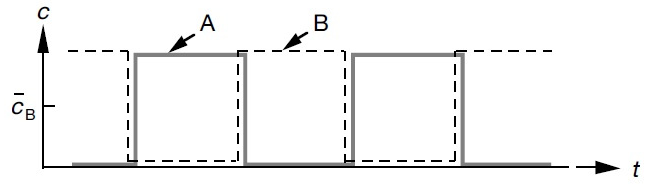
\includegraphics[width=0.6\textwidth]{ReactionRate} 
		%\caption{}
		%\label{fig:}
	\end{figure}
	
	The instantaneous reaction rate is 
	
	\begin{equation}
	\dot{\omega}_{i}= -k_R c_Ac_B=0
	\end{equation}
	
	and the mean (or filtered) reaction rate is $\overline{\dot{\omega}}_{i} = 0$.
}

\frame{\frametitle{The mean (of filtered) Reaction Rate}
	If one attempts to calculate the mean reaction rate replacing the average of the product of the concentrations by the product of the average concentrations it yields
	
	\begin{equation}
	\overline{\dot{\omega}_{i}}= -k_R \overline{ c_Ac_B} =-k_R\left(\overline{c_A} . \overline{c_B}+ \overline{c_{A}^{'}c_{B}^{'}}\right) \neq k_R\left(\overline{c_A} . \overline{c_B} \right)
	\end{equation}
	
}


\frame{\frametitle{The mean (of filtered) Reaction Rate} 
	
	Como a taxa de reação é não linear, modelar os 
	termos $\dot\omega_k$ não é simplesmente expressá-lo
	como uma função das quantidades filtradas $\widetilde Y_F$, $\widetilde Y_O$ e $\widetilde T$. Por meio de uma expansão em série de Taylor, obtem-se
	
	\begin{align}\label{apt4}
	\widetilde{\dot{\omega}}_F = -A \bar\rho^2 \widetilde{T}^\alpha \widetilde Y_F \widetilde Y_O \exp\left(\frac{-T_a}{\widetilde T}\right)
	\left[ 1 + \frac{Y_O^{''}}{\widetilde Y_O} + \frac{Y_F^{''}}{\widetilde Y_F} + \frac{Y_F^{''}Y_O^{''}}{\widetilde Y_O\widetilde Y_F} + \right. \nonumber \\
	(P_1 + Q_1)\left(\frac{T^{''}}{\widetilde T} + \frac{Y_F^{''}T^{''}}{\widetilde T\widetilde Y_F} + \frac{T^{''}Y_O^{''}}
	{\widetilde Y_O\widetilde T} + \frac{T^{''}Y_F^{''}Y_O^{''}}{\widetilde T\widetilde Y_F\widetilde Y_O}\right) \nonumber \\
	\left . + (P_2 + P_1Q_1 + Q_2) \left(\frac{T^{''2}}{\widetilde T^2}  + \frac{Y_F^{''}T^{''2}}{\widetilde T^2\widetilde Y_F} + \frac{T^{''2}Y_O^{''}}
	{\widetilde Y_O\widetilde T^2} + \frac{T^{''2}Y_F^{''}Y_O^{''}}{\widetilde T^2\widetilde Y_F\widetilde Y_O}\right) +\ldots \right]
	\end{align}
	
}


\frame{\frametitle{The mean (of filtered) Reaction Rate} 
	
	Após filtrar a temperatura, $T = \widetilde T + T^{''}$, dada uma função $f(T)$ tem-se que $f(T) = f(\widetilde T + T^{''})$. 
	Expandindo $f(T)$ em série de Taylor obtem-se 
	
	\begin{equation}\label{apt5}
	f(T) = f(\widetilde T + T^{''}) = f(\widetilde T) + T^{''}f_{\widetilde T}(\widetilde T) + \frac{T^{''2}}{2}f_{\widetilde T\widetilde T}
	(\widetilde T) + O(T^{''3}),
	\end{equation}
	
}

\frame{\frametitle{The mean (of filtered) Reaction Rate} 
	
	Assim, os termos $T^{\alpha}$ e $\exp(-T_a/T)$ após a filtragem são substituidos, respectivamente por 
	
	\begin{equation*}\label{apt6}
	T^\alpha = \widetilde T^{\alpha}\left(1+\sum_{n=1}^\infty Q_n\frac{T^{''n}}{\widetilde T^n}\right) 
	= \widetilde T^{\alpha}\left(1+ \alpha\frac{T^{''}}{\widetilde T} + \frac{\alpha(\alpha-1)}{2}\frac{T^{''2}}{\widetilde T^2} + O(T^{''3})\right), 
	\end{equation*}
	
	\begin{align*}
	\exp\left(\frac{-T_a}{T}\right) &= \exp\left(\frac{-T_a}{\widetilde T}\right)\left(1+\sum_{n=1}^\infty P_n\frac{T^{''n}}{\widetilde T^n}\right) \\
	&= \exp\left(\frac{-T_a}{\widetilde T}\right)\left[1 + \frac{T_a}{\widetilde T}\frac{T^{''}}{\widetilde T} + \left(\frac{T_a^2}{\widetilde T^4} -2
	\frac{T_a}{\widetilde T^3}\right)\frac{T^{''2}}{2} + O(T^{''3})\right), 
	\end{align*}

	onde $Q_n$ e $P_n$ são dados pelas expressões
	\begin{equation*}\label{apt7}
	\begin{array}{lll}
	Q_n=\dfrac{1}{n!}\prod_{k=1}^n(\alpha-k-n)& \mbox{ e } & P_n=\sum_{k=1}^n\dfrac{(n-1)!}{(n-k)![(k-1)!]^2k}\left(\dfrac{T_a}{\widetilde T}\right)^n.\\ \\
	\end{array}
	\end{equation*}
	
}


\frame{\frametitle{The mean (of filtered) Reaction Rate} 
	
	So, the replacement of instantaneous values by its mean value, is valid only if
	
	\begin{equation}
	\frac{T_a.T^{''}}{\widetilde{T}^{2}} << 1
	\end{equation}
	
	Typical values of the activation temperature, $T_a=15000, \widetilde{T}=1500$ would limit the temperature fluctuation 
	\begin{equation}
	\frac{15000.T^{''}}{{1500}^{2}} = 1
	\end{equation}
	on $T^{''}=150 $ or $10\%$ of the mean value. In technical combustion process, fluctuations about $70\% $ are observed.
	
	Therefore a statistical description of the turbulence is required. Here we use the Presumed $\beta -PDF$ approach.
}



\frame{\frametitle{Favre decomposition} 

	Carring out the Favre-decomposition for the mass fraction of specie $k$ and modeling the unkown terms, one has
	
	\begin{equation}
	\frac{\partial \bar{\rho} \widetilde{Y_{k}}}{\partial t}+\frac{\partial \bar{\rho} \widetilde{Y_{k}} \widetilde{u_{j}}}{\partial x_{j}}=\frac{\partial}{\partial x_{j}} \left( \rho D_{k} \frac{\partial \widetilde{Y_{k}}}{\partial x_{j}}\right)+\widetilde{\dot{\omega}_{k}} ,
	\label{eq:Especiefavre}
	\end{equation}
	and for the mixture fraction
	
	\begin{equation}
	\frac{\partial \bar{\rho} \widetilde{f}}{\partial t}+\frac{\partial \bar{\rho} \widetilde{f} \widetilde{u_{j}}}{\partial x_{j}}=\frac{\partial}{\partial x_{j}} \left( \rho D_{t} \frac{\partial \widetilde{f}}{\partial x_{j}}\right);
	\end{equation}
	
}

\frame{\frametitle{Favre decomposition} 

	A transport equation for the Favre averaged variance of the mixture fraction can be obtained as
	
	\begin{equation}
	\frac{\partial \overline{\rho} {\widetilde{f^{''2}}} }{\partial t} 
	+ \frac{\partial \overline{\rho} \widetilde{u_i}\widetilde{f^{''2}}}{\partial x_i}
	- \frac{\partial}{\partial x_i}\left( \rho D_{t} \frac{\partial \widetilde{f^{''2}}}{\partial x_{j}}\right)
	= C_{g,1}\overline{\rho}D_{\textit{Eff}}\left|\frac{\partial \widetilde{f}}{\partial x_i}\right|^2 C_{g,2}\overline{\rho}\frac{\varepsilon}{k}\widetilde{f^{''2}}
	\label{eq:fvarEquation}
	\end{equation}
	
	where $D_{\textit{Eff}}$ is the effective coeficient of difusivity, including the turbulence effect. $C_{g,1} = 2.8$ e $C_{g,2} = 2$.
	
	The Favre averaged absolute enthalpy equation reads
	
	\begin{equation}
	\frac{\partial \bar{\rho} \widetilde{h}}{\partial t}+\frac{\partial \bar{\rho} \widetilde{h} \widetilde{u_{j}}}{\partial x_{j}}=\frac{\partial}{\partial x_{j}}\left( \frac{\mu_{t}}{\sigma_{t}} \frac{\partial \widetilde{h}}{\partial x_{j}}\right) ,
	\label{eq:Entalpiafavre}
	\end{equation}
	
}

\begin{frame}[b]{Considerações finais}
	\vfill
	\begin{beamercolorbox}[wd=\textwidth,rounded=true,shadow=true]{block body example}
		\vfill
		\centering \textbf{Perguntas?}
		\vspace*{10pt}
	\end{beamercolorbox}
	\vfill
	\doclicenseThis
\end{frame}

%\frame{\frametitle{Results Nonpremixed flame - D LES - FGM} 
%	% type here the content of the frame
%	
%	\begin{figure}[tbp]
%		\centering
%		%\includegraphics[angle=-0,origin=c,width=0.55\textwidth]{SandiaFlameD_centerline_temperature.png} 
%		\caption{Flame D - Temperature at centreline LES-FGM}
%		\label{fig:perfilchama}
%	\end{figure}
%	
%}




%\begin{frame}{}
%	\centering
%	\Huge Thank you!
%	\vspace{2cm}
%	
%	\normalsize Contact: guenther$@$usp.br
%\end{frame}



\end{document}